


\section{Six Sigma Approaches}
% Fundamentals and Handbook for process management
The first set of analysation and optimization techniques discussed in this chapter originate from the Six Sigma initiative. The name Six Sigma originates from the interval of $6\sigma$ in the normal distribution that indicates the aimed success rate of $99.99966\%$ \cite{siha2008business}\cite{vivekananthamoorthy2011lean} . A representation of the statistical meaning can be see in figure \ref{fig:six-sigma}. Apart from the goal to decrease the error rate, $6\sigma$ is also an methodology for systematically improving process quality \cite{tennant2017six}.

\begin{figure}[H]
		\centering
		\includegraphics[width=0.7\columnwidth]{graphics/six-sigma}
		\caption{The standard normal distribution showing the $6\sigma$ interval (graphic from \cite{vivekananthamoorthy2011lean})} 
		\label{fig:six-sigma} 
\end{figure}

Applied in the context of (executable) business processes, Six Sigma provides a set of methods to identify and eliminate inefficient or needless steps in a process \cite{vom2014handbook}. While countless tools are available as part of Six Sigma, the two main methodologies applied in these tools are \gls{DMAIC}, used for improving existing processes, and \gls{DMADV}, used when creating new processes \cite{selvi2014six} .


In the following, a few selected Six Sigma methods are described that apply the \textbf{DMAIC} and  \textbf{DMADV} approach, these being:  
\begin{itemize}
	\item SIPOC Analysis
	\item Check Sheets
	\item Cause and Effect Diagram
	\item Root Cause Analysis
	\item Quality Function Deployment (QFD)
\end{itemize}

To demonstrate a few of the following methodologies, the exemplary \textit{Missing Part Process} will be used. The fictional process demonstrates what happens when a customer of a furniture shop reports a missing part in his/her order and requests a new part to be shipped. The corresponding \gls{bpmn}-model is shown in Figure \ref{fig:missing-part-process}

\begin{figure}[H]
	\centering
	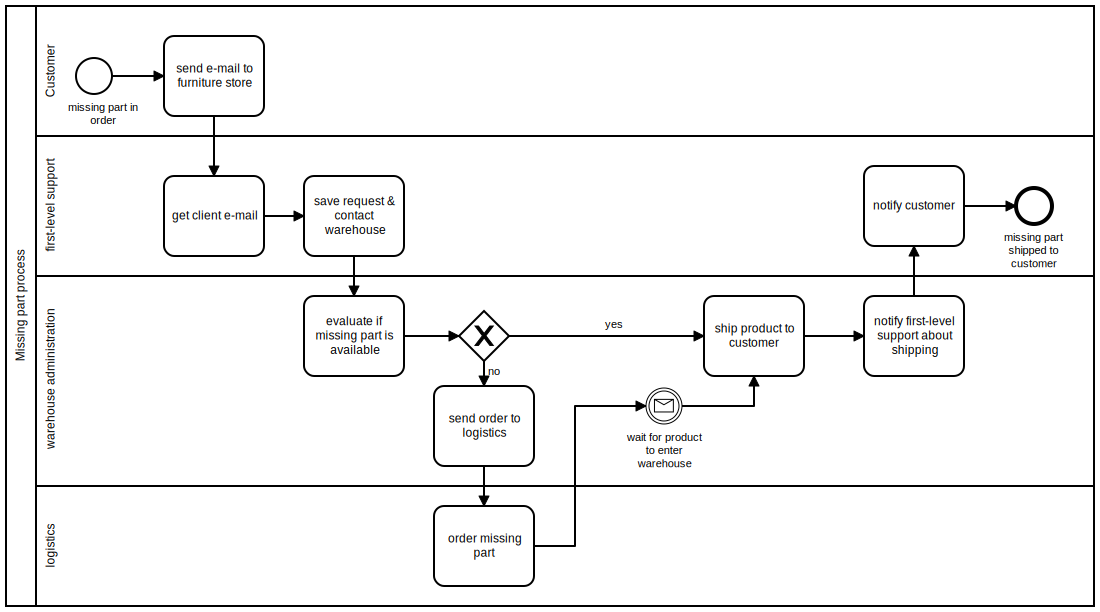
\includegraphics[width=1\columnwidth]{processes/missing-parts-process/missing-parts-process}
	\caption{The \gls{bpmn} model for the \textit{Missing Part Process}} 
	\label{fig:missing-part-process} 
\end{figure}

\subsection{SIPOC Analysis}
The SIPOC analysis is a tool used in the \textbf{Define} phase of \gls{DMAIC} and \gls{DMADV} and should provide more detailed information about each process step than the \gls{bpmn} model  \cite{vom2014handbook}. 

The outcome of a SIPOC analysis is a table, containing the following information for each task in the process \cite{toutenburg2008six}: 
\begin{itemize}
	\item \textbf{S}upplier: provides the input for this task and influence the output the supplier can be internal or external. 
	\item \textbf{I}nput: Resources, data or material needed for this task provided by the suppliers. 
	\item \textbf{P}rocess: the series of actions taken in this task. This can also be a subprocess. 
	\item \textbf{O}utput: represent the result of this process task and provide value for the customer
	\item \textbf{C}ustomer: the customer that benefits from the output of this task (can be external or internal of the organization)
\end{itemize}

When this method is applied to the \textbf{Missing Part Process} the resulting SIPOC table looks like this: 
%TODO Process


\subsection{Check Sheets}

\subsection{Pareto Analysis}

\subsection{Cause and Effect Diagram}

\subsection{Root Cause Analysis}

\subsection{Quality Function Deployment (QFD)}

\section{Other Qualitative Measures}

\subsection{Value Added Analysis (VAA)}


\section{Quantitative Analysis}
The issue with qualitative methods for process improvement is the inability to quantify the impact of theyr application. In order to measure and justify changes in the status quo process we need quantitative methods for analyzing processes. In the context of \gls{bpm}, assessable measures about three different dimensions of a process can be investigated : The process as a whole, resources involved in the process and individual Tasks in a process. \cite{fundamentals}

Before discussing methods for measuring process performance, it is necessary to define what is measured. The four key performance measures examined in this chapter are: cost, time, quality and flexibility. \cite{fundamentals}

The following chapter will present methods for qualitative analysis of processes. Starting with the definition of the four dimensions of process performance: cost, time, quality and flexibility. Afterwards the following methods for measuring performance will be described: 

\begin{itemize}
	\item Flow Analysis
	\item Queues
	\item Simulation
\end{itemize}
\subsection{Performance Measures}
As mentioned above, the performance of a process can be measured using the four dimensions:  cost, time, quality and flexibility. 
\paragraph{Cost}~\\

\paragraph{Time}~\\
\textit{Cycle time} or \textit{throughput time} is the time it takes for a process from start to finish \cite{Six-sigma-terms}. In the case of the \textit{Missing Part Process} shown in \ref{fig:missing-part-process}, the cycle time would be the time that elapses from the moment the customer notices that a part is missing to the time the missing Part is shipped. While the \textit{Cycle time} of the whole process as a metric is highly relevant for client satisfaction, it is on its own usually not tangible when it comes to improvement of the process. The \textit{cycle time} usually consists of two constituents \cite{fundamentals}:
\begin{itemize}
	\item \textit{Processing time}: The time where the request is actively processed, meaning the process participants (e.g. people or software) actually spend this time handling the process. 
	\item \textit{Waiting time}: The time a process spends waiting. Waiting time includes the time the process is waiting in a queue for resources to finish the processing of previous processes and other waiting times, like waiting for the product to enter the warehouse in the \textit{Missing Part Process}
\end{itemize}
\paragraph{Quality}~\\

\paragraph{Flexibility}~\\

\subsection{Flow Analysis}
The Idea behind (work)flow analysis is to estimate the overall performance of a process given the performance of individual tasks.  

Flow analysis is especially useful in order to analyze alternative process designs. By considering the performance of each step in the process, the benefit of process redesigns can be quantified and the impact of automating individual tasks becomes visible.

In the following the analyzed performance measure that is looked at will be execution time. 
\paragraph{Sequential Tasks}~\\
The first calculation starts with sequential tasks or blocks. The execution time of consecutive tasks in a process can be added together to calculate the total time of those two tasks. 
Considering the tasks in \ref{fig:sequential-tasks} where the runtime of each task is brackets below the task name, this would result in a process time of 30s for this block. \cite{ha2006approximate} \cite{fundamentals}

\begin{figure}[H]
	\centering
	\includegraphics[width=0.5\columnwidth]{graphics/sequential-tasks}
	\caption{a process with two sequential executed tasks} 
	\label{fig:sequential-tasks} 
\end{figure}

Considering a more general process model $P$ with sequential blocks $B_1,B_2 ... B_n$ the runtime $R_P$ of process $P$ ca be calculated using the formula \ref{eq:sum-seq}. 
\begin{equation}\label{eq:sum-seq}
	R_P = \displaystyle\sum_{i=1}^{n} B_i
\end{equation}

\paragraph{Parallel Tasks}~\\
The cycle time of parallel tasks or blocks can be calculated using the maximum time of the two parallel blocks. Given the parallel block in \ref{fig:parallel-tasks}, this would result in a process time of 20s for this block.\cite{fundamentals}
\begin{figure}[H]
	\centering
	\includegraphics[width=0.5\columnwidth]{graphics/paralell-tasks}
	\caption{a process with two parallel executed tasks} 
	\label{fig:parallel-tasks} 
\end{figure}

Considering a more general process model $P$ with parallel blocks $B_1,B_2 ... B_n$ the runtime $R_P$ of process $P$ ca be calculated using the formula \ref{eq:sum-par}. 
\begin{equation}\label{eq:sum-par}
	R_P = \operatorname*{arg\,max}_i B_i
\end{equation}

\paragraph{Alternative Sequence Flows}~\\
When having two or more alternative sequence flows with different execution times, additional knowledge about the likelihood of those alternatives is needed \cite{fundamentals}. When looked at the alternative executed tasks in \ref{fig:alternative-tasks}, the average cycle time can be estimated by multiplying the probability of the two alternatives with the execution time of the tasks and summing up the results. This results in $10 * 70\% + 20 * 30\% = 13s$ estimated execution time. 

\begin{figure}[H]
	\centering
	\includegraphics[width=0.5\columnwidth]{graphics/alternative-tasks}
	\caption{a process with two alternative sequence flows} 
	\label{fig:alternative-tasks} 
\end{figure}

Generally, the cycle time $R_P$ of a process $P$ with one or more alternative blocks, that have the runtimes $B_1,B_2 ... B_n$ and a likelihood of $p_1,p_2 ... p_n$ respectively, is estimated with the formula \ref{eq:alternative-seq}. \cite{fundamentals}

\begin{equation}\label{eq:alternative-seq}
	R_P = \displaystyle\sum_{i=1}^{n} B_i * p_i
\end{equation}

\paragraph{Repeating Tasks}~\\
According to the BPMN-Standard\cite{bpmnstandard} defined by OMG, there are multiple ways to indicate that a task or sequence is executed more than once: 

\begin{itemize}
	
	\item \textbf{Multiple Instances}: Three lines in the bottom of the task indicate that a task is executed multiple times - once for every instance or element. There are two kinds of muli-instance tasks, sequential, meaning the instances are processes one after another and parallel, meaning the instances are processed at the same time. 
	\begin{figure}[H]
		\centering
		\includegraphics[width=0.4\columnwidth]{graphics/multi-instance-tasks}
		\caption{Multiple Instance Tasks} 
		\label{fig:muliti-instance-tasks} 
	\end{figure}
	The execution time of these tasks can be estimated using the same calculations as described above with parallel and sequential tasks.
	
	Having a Process $P$ consisting of only one multi-instance task with the runtimes $B_1,B_2 ... B_n$ for each instance, the total runtime $R_P$ of process $P$ ca be calculated using the formula \ref{eq:sum-par} when the instances are executed parallel and \ref{eq:sum-seq} when the instances are executed sequential. 

	\item \textbf{Activity Looping}: A loop in the bottom center of the activity indicates, that this task si performed more than once. The definition on when this task repeats is specified in the \textit{loopCharacteristics}-XML Element.
	\begin{figure}[H]
		\centering
		\includegraphics[width=0.2\columnwidth]{graphics/looped-task}
		\caption{A Task with Activity Looping} 
		\label{fig:activity-looping} 
	\end{figure}
	\item \textbf{Sequence Flow Looping}: Whenever a whole sequence flow instead of a task needs to be repeated, a \textit{Sequence Flow Looping}-pattern can be used where the looping condition is defined within a exclusive gateway. The default flow points back to the start of the repeating sequence flow. 
	\begin{figure}[H]
		\centering
		\includegraphics[width=0.9\columnwidth]{graphics/sequence-flow-looping}
		\caption{The Sequence Flow Looping Pattern} 
		\label{fig:sequence-flow-looping} 
	\end{figure}

	The execution time of both \textbf{Sequence Flow Looping} sequences and \textbf{Activity Looping} tasks are dependent on the probability that these sequences are repeated. Looking at the two equivalent processes in \ref{fig:repeated-example} the probability of Task A repeating is 20\% for each loop taken. Task A is always executed at least once. The probability for Task A being executed twice is $20\% = 0.2$. The probability of Task A being executed three times is $0.2 * 0.2 = 0.04$. Following this pattern, the execution time can be estimated with the infinite sum $
	\displaystyle\sum_{i=1}^{\infty} 0.2^i * 10s$
	

	\begin{figure}[H]
		\centering
		\includegraphics[width=0.9\columnwidth]{graphics/repeated-example}
		\caption{a process with sequence flow looping (left) and the equivalent using activity looping (right)} 
		\label{fig:repeated-example} 
	\end{figure}
\end{itemize}

The exe


% Cycle time using flow analysis
%	additive when sequential
%	Gates:
%		OR: percentage of when option ab and B is used
%		paralell: maximum of the two options
%		inclusive: more complicated....
%	
% 	Cycle time efficnecy : how much time is being waited / can we reduce it
%	Littles Law
%	empirical vs. estimated data



\subsection{Queues}
%see https://link.springer.com/content/pdf/10.1007/11837862.pdf:
%An Approximate Analysis of Expected Cycle Time in Business Process Execution
As mentioned before, the \gls{cycle-time} of a process consists of the time the process is actively executed (\textit{processing time}) and the time the process spends waiting (\textit{waiting time}). In the previous section basic flow analysis was introduced to approximate and analyze these measures.  
While the processing time can be approximated using basic flow analysis, getting an idea about the total expected waiting time of a process is more complex, since flow analysis as it is has no tool to estimate queuing time. 

In order to bridge this gap, the flow analysis can be extended using an queuing approximation algorithm as it is described in this paper\cite{ha2006approximate}.

% TOOD describe flow analysis with queuing analysis

\subsection{Simulation}


\subsection{Cycle Time Efficiency}
\subsection{Littles Law}
\section{Benchmarking Processes}


%H. Harrington - Business Process Improvement chapter 9 